\chapter{Background}

\section{Spintronics}

Nearly five thousand years ago, people already discovered the natural magnets and they found out that when you move two magnets closer to each other, they can either be attractive or repulsive depending on the relative directions. Without understanding the mechanism, people already made some useful stuff such as a horseshoe magnet\cite{wiki:Ferromagnetism}.

\begin{figure}[!ht]
\centering
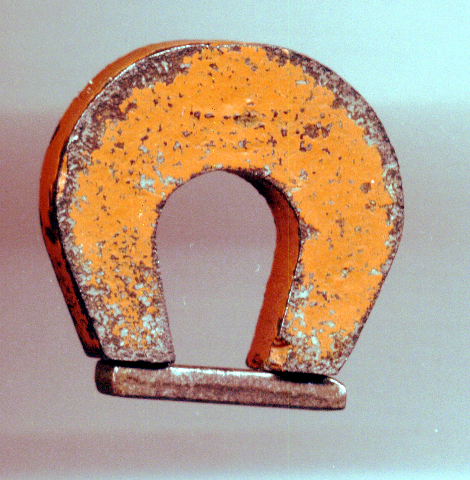
\includegraphics[width=0.3\textwidth]{fig/Magnet.jpg}
\label{Magnet}
\caption{A magnet made of alnico, an iron alloy, with its keeper.}
\end{figure}

However, it was not until 1925 that the underlying mystery of ferromagntism started to reveal itself. George Uhlenbeck and Samuel Goudsmit proposed the idea that each electron spins with an angular momentum of one half Planck constant and carries a magnetic moment of one Bohr magneton. Even though the famous Hendrik Lorentz pointed out that the idea of a spinning electron would be incompatible with classical electrodynamics, those two physicists went ahead and published their results. Of course, they were right and Lorentz was wrong. Uhlenbeck and Goudsmit maybe could not image their findings to have such a great impact on modern information technology. While electronics, the manipulations of electron charges in various kinds of devices, has been developed greatly since 1950s and shaped a new world, the development of spintronics started to influence the modern technology since 1980s. Johnson and Silsbee\cite{JohnsonandSilsbee} observed spin-polarized electron injection from a ferromagnetic metal to a normal metal.  Albert Fert\cite{Fert} and Peter Gr\"unberg\cite{Grunberg} independently discovered the phenomena of Giant magnetoresistance(GMR) and they have been rewarded The Nobel Prize in Physics 2007 for the practise significance of this work. Spintronics have several major advantages over conventional electronics. Unlike the conventional electronics which relies on the transportation of electrons charges, which inevitably creates heating dissipation and power loss, spintronics can perform with pure spin currents and movements of spin angular momentum without heat. Moreover, once formed, the spins does not need energy to maintain it. The non-volatility takes a huge advantages in static power consumption. Spintronics has a great ongoing and potential applications in memory storage, signal processing and logical devices.

\section{Tunnel Magnetoresistance}

The Tunnel Magnetoresistance effect\cite{TMR} refers to the change of resistance of a ferromagnetic/non-magnetic barrier/ferromagnetic metallic multilayer structure as the relative orientation of the magnetizations of two ferromagnetic layers changes. When the two layers have parallel magnetizations, the resistance is lowest and the resistance is maximum when magnetizations of two ferromagnetic layers are anti-parallel. Nowadays, the resistance difference between the maximum and minimum values can be as much as 100 per cent.

We first consider a simple case when electrons are passing through a single ferromagnetic layer. For a 3d transitional ferromagnetic layer like Ni, Co and Fe, ferromagnetism is coming from the exchange coupling of 3d electrons. In a simplified band structure for ferromagnetic metals, the exchange coupling results in an split of energy band for 3d electrons. As a result when the spin-up band and spin-down band are filled up to the Fermi level, there will be more spin-up electrons than spin-down electrons, which induces a net magnetization. On the other hand, the majority and minority spin bands also have different density of states at the Fermi level. The conduction properties of a metal are primarily determined by the electrons near the Fermi level. When spin unpolarized electrons consisting of equal numbers of spin-up and spin-down electrons travel in a ferromagnet, different spins experiences different resistances. Besides, different types of spins also experience different scattering at the interface due to the band structure mismatch. Overall, one type of spins has higher probability to transmit through than the other type.

\begin{figure}[!ht]
\centering
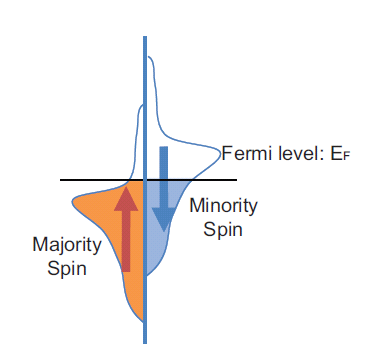
\includegraphics{fig/Fermi.PNG}
\label{Fermi}
\caption{Band structure for ferromagnet. Due to energy split, the majority and minority spin bands have different of states at the Fermi level.}

\end{figure}




Now, we have two magnetic layers separated by a tunnel barrier. As it has been proposed by Julliere in 1975, the tunneling probability across the tunnel barrier,which can be treated as conductance in this case, is proportional to the density of states of both initial and final states. Then we have 




\begin{figure}[!ht]
\centering
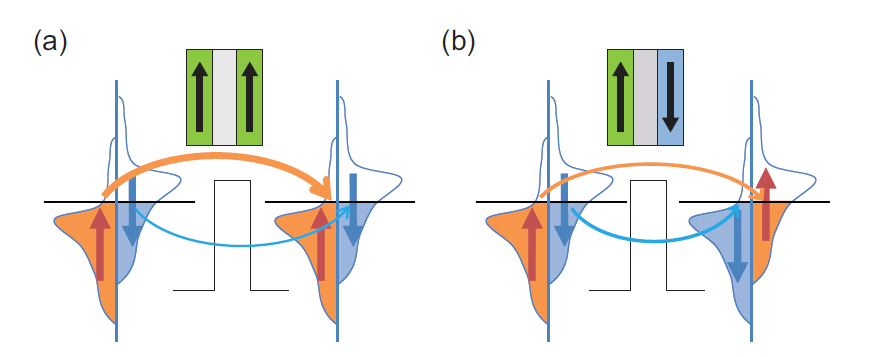
\includegraphics[width=1.0\textwidth]{fig/TMR.PNG}
\label{TMR}
\caption{Illustration of tunnel magnetoresistance effect. (a)Configuration of two layers are parallel.(b)Configurations of two layers are anti-parallel.}
\end{figure}


\begin{equation}
\label{eq:conductance}
\begin{aligned}
G_{p} &\propto  \rho_{L\uparrow}\rho_{R\uparrow}  + \rho_{L\downarrow}\rho_{R\downarrow}
\\
G_{Ap} &\propto  \rho_{L\uparrow}\rho_{R\downarrow}  + \rho_{L\downarrow}\rho_{R\uparrow}
\end{aligned}
\end{equation}


where $G_P$($G_{AP}$) is the parallel(anti-parallel) conductance, $\rho_{L\uparrow}$ and$\rho_{L\downarrow}$($\rho_{R\uparrow}$ and$\rho_{R\downarrow}$) are densities of states for up and down spins of the left(right) ferromagnet. By definition, the spin polarization P is 
\begin{equation}
P = \frac{\rho_{\uparrow} - \rho_{\downarrow}} {\rho_{\uparrow} + \rho_{\downarrow}}
\end{equation}

Therefore the tunnel magnetoresistance ratio can be calculated as

\begin{equation}
TMR = \frac{R_{AP} - R_{P}}{R_{P}}= \frac{G_{P} - G_{AP}}{G_{AP}} = \frac{2P_LP_R}{1-P_LP_R}
\end{equation}

In early studies of MTJs,a TMR ratio of a few 10's of percent was achieved with amorphous aluminum oxide(AlO)barries. Most recently, single crystalline magnesium oxide(MgO) barries were predicted to provide a much higher TMR ratio due to the wavefunction match between the ferromagnetic electrodes and the tunnel barrier. TMR ratios of around 200 percent were then demonstrated and led to intensive studies in MgO bases MTJs mainly because of the high TMR ratio founded in this family\cite{Mg0}.


\section{Spin transfer torque}

Spin transfer torque refers to the torque between electrons and local magnetization. As it is shown in \ref{fig:electron}, the direction of incident electron is randomly distributed in all directions. When electrons are entering a ferromagnetic layer, due to the fixed magnetization of this FM layer, electrons are parallel to the local magnetization will have high probability of transmission and on the other hand, the electrons having opposite direction will mostly be reflected. As a result, transmitted electrons will be aligned to the local magnetization and reflected. In this process, the angular momentum of incident electrons has been changed by local magnetization. On the other hand, the local magnetization also experience torque from incident electrons as well. This torque is called the spin transfer torque\cite{STT} \cite{Currenttorque} and can provide an efficient way to manipulate local magnetization as we shall see next.

\begin{figure}[ht]

  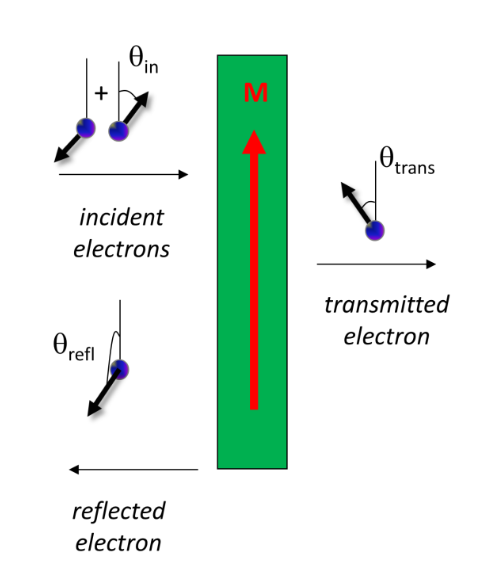
\includegraphics[width=60mm]{fig/electron.png}
  \centering
  \caption{Schematic of electrons transmitting through and getting reflected from ferromagnet metal, with the transverse spin component absorbed during the process.  }
  \label{fig:electron}
\end{figure}

Magnetic tunnel junction is the main device we have been studied. The device has a a structure of two ferromagnetic layers separated by a spacer. The mulitilayers are patterned into a elliptically-shaped nanopillar withe size normally around 60nm. The top and bottom of the devices are connected to electrical leads to allow current to pass perpendicularly through the multilayers.

The dynamics of the magnetization in the presence of spin transfer torque can be described by the classical Landau-Lifshitz-Gilbert(LLG) equation including an additional term for the spin torque:

\begin{equation}
\frac{dM}{dt} = \gamma M \times H_{eff} + \alpha M \times \frac{dM}{dt} + g(\theta)\frac{\gamma \hbar I}{eV_{free}M_s}M \times(M \times M_{fix})
\end{equation}

where $H_{eff}$ is the total effective field including the applied field $H_{applied}$ and the anisotropy field $H_{ani}$ and $\alpha$ is the damping constant. The first term is the field torque term which makes the magnetization precess around the effective field direction. The second term is the damping torque which relates the energy dissipation. On average it points towards the equilibrium position of the magnetization, so that without any external excitation the magnetization will relax back to the equilibrium. The third term is the spin transfer torque. The direction of this torque depends on the direction of the electron flow. For electron flow from the fixed layer to the free layer, this torque is in the same direction as the damping torque assuming the fixed layer also along the effective field direction, in this case spin transfer torque works as additional damping torque. On the other hand, for electron flow from the free layer to the fixed layer, this torque works against the damping torque and thus can reduce the relaxation.

The first case we discussed is of less interest. For the second case we have the competition between spin transfer torque and damping torque\cite{Bias}. Usually the spin transfer torque is small compared to the field torque. So the effect of spin transfer torque can be viewed as either increasing or decreasing the amplitude of the magnetic precession. In general, the magnetic dynamics excited by spin transfer torque can be categorized in to two types: switching and persistent precession.

\begin{figure}[h!]
\centering
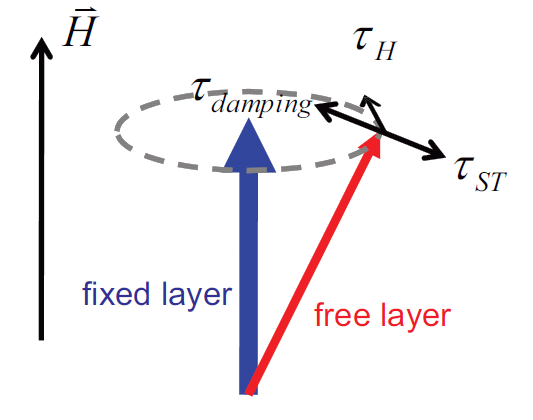
\includegraphics[width=0.5\textwidth]{fig/dampingtorque.PNG}
\label{Torque}
\caption{Direction of torques presented in the system.}

\end{figure}

\section{Magnetic Tunnel Junctions with Perpendicular Magnetic Anisotropy}

\subsection{Critical Switching Voltage}

In this section we would like to derive the critical switching voltage of the Magnetic Tunnel Junction(MTJ). We would like to prove that the critical voltage is symmetric between the Anti-Parallel state and the Parallel state, which is an important reason why it is crucial to characterize the MTJ in terms of bias voltage, not the bias current as used in many other magnetic materials system.

The critical switching current is given by\cite{SlonSwitching}
\begin{equation}
    I_{c0} = 2 \alpha \frac{\gamma e}{\mu_B \eta}E
\end{equation}
Here $\alpha$ is the Gilbert damping constant , $\gamma$ is gyromagnetic ratio, e is the elementary charge  $\eta$ is the spin-transfer efficiency. The energy barrier $E$ is given by
\begin{equation}
    E = M_s H_K V / 2
\end{equation}
Here $M_s$ is the saturation magnetization, $H_K$ the anisotropy field, V is the volume. We can further rewrite the spin transfer efficiency as
\begin{equation}
    \eta = \frac{P}{2}\frac{1}{1+P^2 \cos{\theta}}
\end{equation}

P is the polarization factor given by
\begin{equation}
    P = \sqrt{\frac{G_P - G_{AP}}{ G_P + G_{AP}} }       
\end{equation}
The conductance of the Magnetic Tunnel Junction can be given by\cite{MTJConductance}
\begin{equation}
    G(\theta) = \frac{1}{2} (G_P + G_{AP}) + \frac{1}{2} (G_P - G_{AP}) \cos{\theta}
    = \frac{G_P + G_{AP}}{2}\big[ 1+P^2\cos{\theta} \big]
\end{equation}
If we define $G_0 = \frac{G_P + G_{AP}}{2}$ as the average conductance and use the Ohm's Law, the critical switching voltage for MTJ should be
\begin{equation}
    V_{C0} = \frac{I_{C0}}{G(\theta)} = 2\alpha\frac{\gamma e}{\mu_B}E\frac{1}{\eta G(\theta)}
\end{equation}
Replacing gyromagnetic ratio with g factor $\gamma = \frac{g \mu_B}{\hbar}$, the above equation becomes
\begin{equation}
    \label{eq:criticalV}
    V_{C0} = 4\alpha\frac{ge}{\hbar P G_0}E
\end{equation}

One can easily find from Eq.\ref{eq:criticalV}, it is clear that the critical switching voltage of MTJs do noes depend on the relative configurations of two ferromagnetic layers of the MTJ. Parral and Anti-Parallel states have the same critical voltage(in this macrospin model).  




\section{Magnetic Switching}

At zero or small field, both direction along the easy axis correspond to local energy minimums so it is possible to switch the magnetization between these two directions with spin transfer torque. For example, for a device with both free and fixed layers keeping at the easy axis direction and parallel to each other, if we flow a positive current defined as current flow from free to fixed layer, according to previous analysis, the spin transfer torque acts on the free layer is pointing away from the fixed layer and destabilizes this configuration so that the magnetic moment of the free layer goes into a precession around the easy axis. If we keep increasing the current, the amplitude of the free layer precession increases until it reaches the energy barrier which is around 90 degree. After the free layer changes direction, now the spin transfer torque will act as damping torque again and stabilize the magnetization. Similarly, if the magnetic tunnel junction starts in the anti-parallel configuration, a strong enough negative current can switch the free layer back to the parallel configuration. If we monitor the resistance of the device, it will exhibit a hysteresis loop as we sweep the current, as shown in the example

\begin{figure}[h!]
\centering
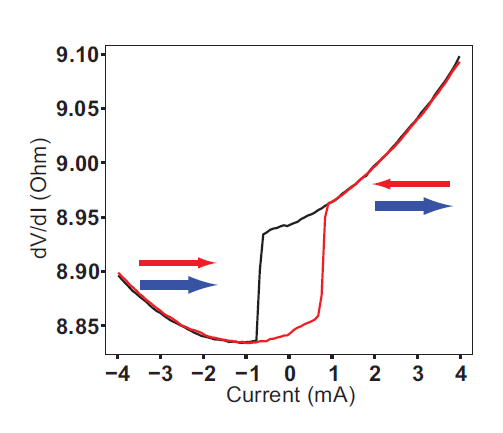
\includegraphics[width=0.5\textwidth]{fig/DC.PNG}
\label{DC}
\caption{Differential resistance with respect to dc current. Arrows indicate magnetic state to be either parallel and anti-parallel.}

\end{figure}

The critical switching current $I_c$ is defined as the current required to achieve switching at zero temperature(no thermal excitations)  . Above $I_c$, the spin torque is stronger than the damping torque and drives the free layer moment to switch direction.[Fig] illustrate the switching process. The switching proceeds via a precessional motion of the magnetization with increasing amplitude\cite{subswitch}. The switching time is defined as the following :


\begin{figure}[!ht]
\centering
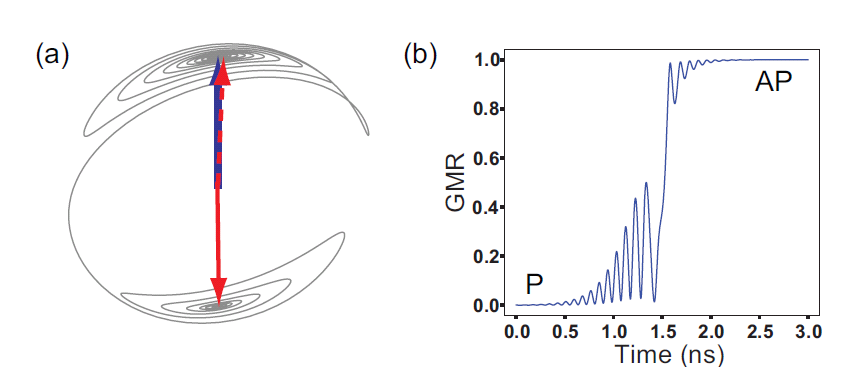
\includegraphics[width=1.0\textwidth]{fig/switching.PNG}
\label{Switching}
\caption{An example of a simulated spin transfer switching event.(a)Switching trajectory. Dotted lines show initial state of free layer. Solid line shows the switching (b) Normalized resistance value as a function of time}
\end{figure}

\begin{equation}
t_s \propto \frac{1}{I-I_c}
\end{equation}

Now if the applied current is smaller than the critical current, the spin torque is not strong enough to drive the free layer moment to directly overcome the energy barrier to achieve switching but only to excite magnetic precession at small amplitudes. At finite temperatures, switching can still occur due to thermal excitations. This thermal-assisted magnetization reversal can be described by the Neel-Brown relaxation time:
\begin{equation}
P(t) = 1 - exp(-t/\tau)
\end{equation}
where t is the observation time, and $\tau$ is the relaxation time which is given by
\begin{equation}
\tau = \frac{1}{f_0}\exp{E_b/k_B T}
\end{equation}
Here $f_0$ is the attempt frequency, $E_b$ is the energy barrier and T is the temperature. Thermal assisted switching can be modeled by a fluctuating field with a Gaussian stochastic process. The relaxation time $\tau$ can be modified as the following:

\begin{equation}
\tau = \frac{1}{f_0}\exp [\frac{E_b}{k_B T}(1 - \frac{I}{I_c})]
\end{equation}


\section{Ferromagnetic Resonance}
We start with the cordinate system that the place $y=0$ is subjected to a d.c. field $H_z$ and a weak microwave field $H_x$. The magnetization $\boldsymbol{M}$ and the angular momentum density $\boldsymbol{J}$ are related by $\boldsymbol{M} = \gamma \boldsymbol{J}$\cite{Kittel1947}\cite{Kittel}, where $\gamma$ is the gyromagnetic ratio. The equation of motion $\frac{\partial J}{\partial t} = \big[\boldsymbol{M} \times \boldsymbol{H}]$ can be written as 
\begin{equation}
    \label{eq:Mmotion}
    \frac{\partial \boldsymbol{M}}{\partial t} = \gamma \big[\boldsymbol{M} \times \boldsymbol{H}]
\end{equation}
If we want to solve for the general resonance condition for a ellipsoid with major axis parallel to the x, y, z axes of the coordinate system, we first have the demagnetization factor: $N_x$,$N_y$ and $N_z$. The effective values of the magnetic field components are
\begin{equation}
\label{eq:MvsT}
\begin{aligned}
{H_x}^i &= H_x - N_x M_x \\
{H_y}^i &=  - N_y M_y \\
{H_z}^i &= H_z - N_z M_z \\
\end{aligned}
\end{equation}

The values ${H_x}^i$  ${H_y}^i$ and ${H_z}^i$ should be used when substituting $H$ in Eq.\ref{eq:Mmotion}. Now we can decompose Eq.\ref{eq:Mmotion} into 

\begin{equation}
\label{eq:MvsT}
\begin{aligned}
\partial M_x \char`\/ \partial t &= \gamma\big[H_z + (N_y - N_z) M_z] M_y   \\
\partial M_y \char`\/ \partial t &= \gamma\big[M_z H_x - (N_x - Nz)M_x M_z - MxHz]   \\
\partial M_z \char`\/ \partial t &\approx 0
\end{aligned}
\end{equation}

If we solve these equations with time dependent $\exp{i \omega t}$, the susceptibility $\chi_x = M_x / H_x$ is given by 

\begin{equation}
    \label{eq:suscept}
    \chi_x = \frac{\chi_0}{1 - (\omega / \omega_0)^2}
\end{equation}

where
\begin{equation}
    \label{eq:chi0}
    \chi_0 = \frac{M_z}{H_z + (N_x - Nz)Mz}
\end{equation}
and the resonance frequency is given by 
\begin{equation}
    \label{eq:resonance}
    \omega_0 = \gamma \big\{ \big[Hz+(N_y - N_z)M_z] \times \big[Hz+(N_x - N_z)M_z]          \big\}^\frac{1}{2}
\end{equation}

From Eq.\ref{eq:resonance} we can have some special cases:
\begin{enumerate}
  \item Plane ($N_x = N_z = 0$;$N_y = 4 \pi$)
  \begin{equation}
      \omega_0 = \gamma (B_z H_z)^\frac{1}{2}
  \end{equation}
  \item Sphere ($N_x = N_y = N_z = 4\pi/3$)
  \begin{equation}
      \omega_0 = \gamma H_z
  \end{equation}
  \item Infinite Circular Cylinder ($N_x = N_y = 2\pi$;$N_z = 0 $)
  \begin{equation}
      \omega_0 = \gamma (H_z+2\pi Mz)
  \end{equation}
\end{enumerate}
It is often that the ferromagnetic crystals energies depends on the relative magnetization orientations and in order to minimize the total energy, the magnetizations would align with the easy axis. This is called the anisotropy energy. If the anisotropy is uniaxial, the first-order magnetic anisotropy can be written as 
\begin{equation}
    f = K_1 {\sin{\theta}}^2
\end{equation}
where f refers to unit volume of material. $\theta$ is the angle between the magnetizations and the easy axis of the crystal. $K_1$ is the first-order anisotropy constant. To account for the effect on resonance conditions, it is easier to consider the effect in terms of an equivalent magnetic field. The equivalent field $H^e$ is defined as
\begin{equation}
    \partial f \char`\/ \partial \theta = M_s \times H^e
\end{equation}
It should be noted that the direction of effective field $H^e$ is still arbitrary and without lose any generality, we can express the effective field in terms of effective demagnetizing factor $N^e$ as
\begin{equation}
    \begin{aligned}
        {H_x}^e &= - {N_x}^e M_x \\
        {H_y}^e &= - {N_y}^e M_y \\
    \end{aligned}
\end{equation}
The resonance condition from Eq.\ref{eq:resonance} can now be modified as 
\begin{equation}
    \label{eq:resonanceKu}
    \omega_0 = \gamma \big\{ \big[Hz+(N_y + {N_y}^e - N_z)M_z] \times \big[Hz+(N_x + {N_x}^e - N_z)M_z]          \big\}^\frac{1}{2}
\end{equation}
I
\section{Spin-torque Ferromagnetic Resonance}

As we mentioned above, when the spin transfer torque is small, the magnetization will not reverse however experience a persistent precession. By applying AC current, excited magnetic precession can be detected by measuring a mixing DC voltage from the product of the resistance oscillation and the ac current. This Spin-transfer Ferromagnetic Resonance (ST-FMR) \cite{Sankey2006}\cite{Tulapurkar2005} is similar to the traditional ferromagnetic resonance, but can be performed in much smaller devices. The ST-FMR technique can be used to characterize important material properties such as voltage-controlled-anisotropy\cite{VCMA1}\cite{Jian}\cite{Wang2012}, magnetic damping\cite{PRLdamping}, field-like torque\cite{Sankey2008} along with the spectrum of magnetic excitations of the MTJ\cite{excitation1}\cite{excitation2}, which is not important for understanding basis physic phenomena like spin-tunnel process but also essential for characterizing and optimizing the MTJs for future applications. In Chapter 3, I will describe an improved technique to measure Spin-torque Ferromagnetic Resonance with field modulations.








